\documentclass[10pt, aspectratio=169]{beamer}

% --- Unicode Support (pdflatex) ---
\usepackage[utf8]{inputenc}
\usepackage[T5]{fontenc}
\usepackage{textcomp}

% --- Theme & Settings ---
\usetheme{metropolis}
\usepackage{booktabs}
\usepackage{graphicx}
\usepackage{amsmath}
\usepackage{amsfonts}
\usepackage{tikz}
\usetikzlibrary{shapes.geometric, arrows.meta, positioning, calc, fit}
\usepackage{pgfplots}
\pgfplotsset{compat=1.17}
\usepackage{multirow}
\usepackage{tabularx}
\renewcommand{\arraystretch}{1.2}

% --- Custom Colors (Strictly Black & White) ---
\setbeamercolor{frametitle}{bg=white, fg=black}
\setbeamercolor{background canvas}{bg=white}
\setbeamercolor{normal text}{fg=black}
\setbeamercolor{section in toc}{fg=black}
\setbeamercolor{block title}{bg=gray!15, fg=black}
\setbeamercolor{block body}{bg=gray!5}

% --- CUSTOM FRAME TITLE ---
\makeatletter
\setbeamertemplate{frametitle}{%
  \nointerlineskip%
  \begin{beamercolorbox}[wd=\paperwidth,ht=5ex,dp=1.9ex,sep=0pt]{frametitle}
    \hspace*{2em}\textbf{\insertframetitle} 
  \end{beamercolorbox}%
  \nointerlineskip%
  \hrule height 0.5pt \relax 
}
\makeatother

% --- Title Information ---
\title{Xây dựng hệ thống Data Warehouse \\ và Phân tích Dữ liệu Bán lẻ Trực tuyến}
\subtitle{Kho Dữ Liệu và Hệ hỗ trợ quyết định --- HCMUT}
\author{\textbf{Phạm Quang Hiếu -- 2310974 \quad Nguyễn Trung Hiếu -- 2310965}}
\institute{GVHD: Bùi Tiến Đức}
\date{Tháng 04/2026}

\begin{document}

\maketitle

% ==========================================
% TABLE OF CONTENTS
% ==========================================
\begin{frame}{Nội dung trình bày}
    \tableofcontents
\end{frame}

% ==========================================
% SECTION 1: INTRODUCTION
% ==========================================
\section{Giới thiệu đề tài}

\begin{frame}{1. Bối cảnh và Động lực}
    \small
    \begin{columns}[T]
        \begin{column}{0.55\textwidth}
            \textbf{Vấn đề:} Doanh nghiệp bán lẻ trực tuyến tạo ra lượng dữ liệu giao dịch khổng lồ nhưng thiếu công cụ khai thác.
            
            \vspace{0.2cm}
            \textbf{Vì sao OLTP không đủ?}
            \begin{itemize}
                \item \textbf{OLTP} tối ưu cho ghi/đọc từng giao dịch.
                \item \textbf{VD:} Truy vấn ``Tổng doanh thu Q4 theo quốc gia'' trên OLTP cần quét toàn bộ bảng $\Rightarrow$ chậm.
                \item \textbf{OLAP} (DW) tổ chức theo chiều phân tích $\Rightarrow$ nhanh hơn hàng chục lần.
            \end{itemize}
        \end{column}
        
        \begin{column}{0.4\textwidth}
            \begin{center}
            \begin{tikzpicture}[scale=0.7, every node/.style={transform shape},
                box/.style={rectangle, draw, thick, text width=2.6cm, align=center, minimum height=0.8cm, rounded corners=2pt}]
                
                \node[box, fill=gray!10] (oltp) at (0,2.2) {\textbf{OLTP}\\Row-oriented\\Low latency writes};
                \node[box, fill=gray!10] (olap) at (0,0) {\textbf{OLAP (DW)}\\Column-oriented\\Fast aggregation};
                
                \draw[-{Stealth}, thick] (oltp) -- (olap) node[midway, right, font=\scriptsize] {ETL};
                
                \node[font=\scriptsize, gray, left=0.3cm of oltp] {Giao dịch};
                \node[font=\scriptsize, gray, left=0.3cm of olap] {Phân tích};
            \end{tikzpicture}
            \end{center}
            
            \vspace{0.1cm}
            \textbf{Giải pháp:} Data Warehouse + BI + Data Mining theo mô hình Kimball.
        \end{column}
    \end{columns}
\end{frame}

\begin{frame}{2. Mục tiêu nghiên cứu}
    \small
    \textbf{Câu hỏi:} Xây dựng hệ thống DW hoàn chỉnh cho bán lẻ, phân tích hành vi và dự đoán giá trị khách hàng?

    \vspace{0.2cm}
    \begin{columns}[T]
        \begin{column}{0.48\textwidth}
            \textbf{6 mục tiêu cụ thể:}
            \begin{enumerate}
                \item Pipeline \textbf{ETL} tự động
                \item Thiết kế \textbf{Star Schema}
                \item Phân cụm KH (\textbf{K-Means + RFM})
                \item Dự đoán CLV (\textbf{XGBoost})
                \item Luật kết hợp SP (\textbf{FP-Growth})
                \item Dashboard (\textbf{Streamlit + Plotly})
            \end{enumerate}
        \end{column}
        
        \begin{column}{0.48\textwidth}
            \textbf{Ý nghĩa thực tiễn:}
            \begin{itemize}
                \item \textbf{Quản trị KH:} Xác định nhóm KH giá trị cao, KH nguy cơ rời bỏ.
                \item \textbf{Dự báo:} CLV giúp lập ngân sách marketing.
                \item \textbf{Tối ưu:} Cross-selling tăng giá trị đơn hàng.
            \end{itemize}
        \end{column}
    \end{columns}
\end{frame}

\begin{frame}{3. Tập dữ liệu --- Online Retail Dataset}
    \small
    \begin{columns}[T]
        \begin{column}{0.42\textwidth}
            \textbf{Nguồn:} Kaggle --- Giao dịch thực tế từ công ty bán lẻ quà tặng tại UK.
            
            \vspace{0.2cm}
            \begin{tabularx}{\linewidth}{lX}
                \toprule
                \textbf{Thuộc tính} & \textbf{Giá trị} \\
                \midrule
                Bản ghi (raw) & 541,909 \\
                Số thuộc tính & 8 \\
                Kích thước & $\sim$46 MB \\
                Giai đoạn & 12/2010 -- 12/2011 \\
                Định dạng & CSV (ISO-8859-1) \\
                \bottomrule
            \end{tabularx}
        \end{column}
        
        \begin{column}{0.54\textwidth}
            \footnotesize
            \begin{tabularx}{\linewidth}{llX}
                \toprule
                \textbf{Cột} & \textbf{Kiểu} & \textbf{Mô tả} \\
                \midrule
                InvoiceNo & String & Mã hóa đơn (C=hủy) \\
                StockCode & String & Mã sản phẩm \\
                Description & String & Tên sản phẩm \\
                Quantity & Integer & Số lượng mua \\
                InvoiceDate & DateTime & Thời gian giao dịch \\
                UnitPrice & Float & Đơn giá (£) \\
                CustomerID & Float & Mã khách hàng \\
                Country & String & Quốc gia \\
                \bottomrule
            \end{tabularx}
        \end{column}
    \end{columns}
\end{frame}

% ==========================================
% SECTION 2: DATA PREPROCESSING
% ==========================================
\section{Data Preprocessing}

\begin{frame}{4. Quy trình làm sạch dữ liệu}
    \small
    \textbf{5 bước tuần tự:} Mỗi bước loại bỏ một loại dữ liệu không hợp lệ.
    
    \vspace{0.15cm}
    \begin{center}
    \resizebox{0.92\textwidth}{!}{
    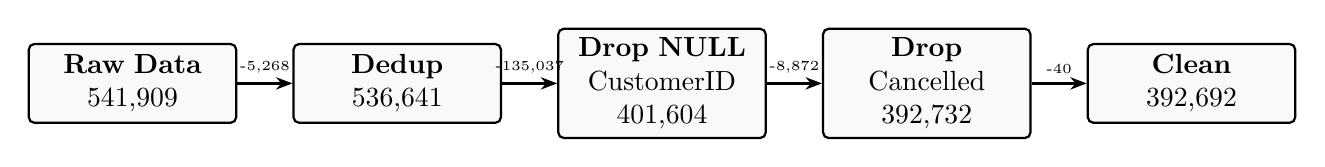
\begin{tikzpicture}[
        node distance=0.15cm and 0.7cm,
        box/.style={rectangle, draw, thick, text width=2.4cm, align=center, minimum height=1cm, rounded corners=2pt, fill=gray!5},
        arrow/.style={-{Stealth[scale=0.9]}, thick}
    ]
        \node[box] (raw) {\textbf{Raw Data}\\541,909};
        \node[box, right=of raw] (dedup) {\textbf{Dedup}\\536,641};
        \node[box, right=of dedup] (cust) {\textbf{Drop NULL}\\CustomerID\\401,604};
        \node[box, right=of cust] (cancel) {\textbf{Drop}\\Cancelled\\392,732};
        \node[box, right=of cancel] (clean) {\textbf{Clean}\\392,692};
        
        \draw[arrow] (raw) -- (dedup) node[midway, above, font=\tiny] {-5,268};
        \draw[arrow] (dedup) -- (cust) node[midway, above, font=\tiny] {-135,037};
        \draw[arrow] (cust) -- (cancel) node[midway, above, font=\tiny] {-8,872};
        \draw[arrow] (cancel) -- (clean) node[midway, above, font=\tiny] {-40};
    \end{tikzpicture}
    }
    \end{center}
    
    \vspace{0.15cm}
    \begin{columns}[T]
        \begin{column}{0.48\textwidth}
            \begin{itemize}
                \item \textbf{Missing CustomerID} ($\sim$25\%): Loại bỏ --- khóa chính cho phân tích RFM.
                \item \textbf{Duplicates:} 5,268 bản ghi trùng lặp.
            \end{itemize}
        \end{column}
        \begin{column}{0.48\textwidth}
            \begin{itemize}
                \item \textbf{Hóa đơn hủy} (InvoiceNo bắt đầu ``C''): Không phản ánh hành vi mua thực tế.
                \item \textbf{Quantity/UnitPrice $\leq$ 0}: Không hợp lệ.
            \end{itemize}
        \end{column}
    \end{columns}
\end{frame}

\begin{frame}{5. Feature Engineering --- Phân tích RFM}
    \small
    \begin{block}{RFM: Phương pháp phân khúc KH kinh điển trong marketing}
    \end{block}
    
    \vspace{0.1cm}
    \begin{columns}[T]
        \begin{column}{0.52\textwidth}
            \begin{itemize}
                \item \textbf{Recency (R):} Số ngày từ lần mua cuối.
                    \\\textit{VD: KH mua 5 ngày trước $\Rightarrow R=5$.}
                \item \textbf{Frequency (F):} Số hóa đơn duy nhất.
                    \\\textit{VD: KH có 10 hóa đơn $\Rightarrow F=10$.}
                \item \textbf{Monetary (M):} Tổng chi tiêu.
                    \\\textit{VD: KH chi £2,500 $\Rightarrow M=2500$.}
            \end{itemize}
            
            \vspace{0.15cm}
            \textbf{Biến tạo thêm:}
            \begin{itemize}
                \item $\text{TotalPrice} = \text{Quantity} \times \text{UnitPrice}$
                \item InvoiceDate $\to$ Year, Month, Quarter
            \end{itemize}
        \end{column}
        
        \begin{column}{0.44\textwidth}
            \textbf{Chuẩn hóa (StandardScaler):}
            $$z = \frac{x - \mu}{\sigma}$$
            
            \textit{Lý do:} RFM phân bố rất lệch (skewed) $\Rightarrow$ z-score giúp K-Means không thiên vị bởi scale.
            
            \vspace{0.15cm}
            \textbf{Encoding (FP-Growth):}\\
            Basket matrix one-hot:\\1 = đã mua, 0 = không mua.
        \end{column}
    \end{columns}
\end{frame}

% ==========================================
% SECTION 3: SYSTEM ARCHITECTURE
% ==========================================
\section{Kiến trúc hệ thống}

\begin{frame}{6. Kiến trúc tổng thể}
    \small
    \begin{center}
    \resizebox{0.9\textwidth}{!}{
    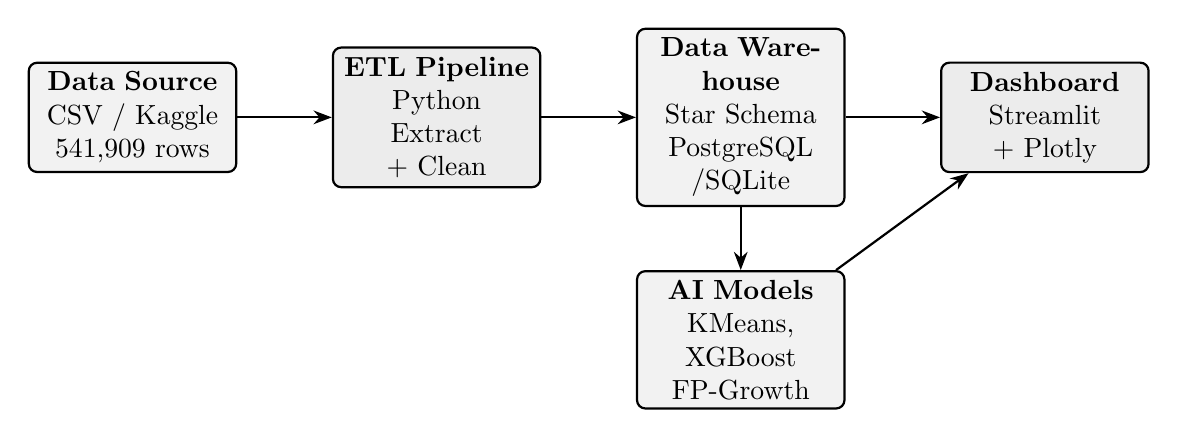
\begin{tikzpicture}[
        node distance=1cm and 1.2cm,
        box/.style={rectangle, draw, thick, text width=2.4cm, align=center, minimum height=1cm, rounded corners=3pt},
        arrow/.style={-{Stealth[scale=1.0]}, thick}
    ]
        \node[box, fill=gray!10] (src) {\textbf{Data Source}\\CSV / Kaggle\\541,909 rows};
        \node[box, fill=gray!15, right=of src] (etl) {\textbf{ETL Pipeline}\\Python\\Extract + Clean};
        \node[box, fill=gray!10, right=of etl] (dw) {\textbf{Data Warehouse}\\Star Schema\\PostgreSQL\\/SQLite};
        \node[box, fill=gray!15, right=of dw] (bi) {\textbf{Dashboard}\\Streamlit + Plotly};
        \node[box, fill=gray!10, below=0.8cm of dw] (ai) {\textbf{AI Models}\\KMeans, XGBoost\\FP-Growth};
        
        \draw[arrow] (src) -- (etl);
        \draw[arrow] (etl) -- (dw);
        \draw[arrow] (dw) -- (bi);
        \draw[arrow] (dw) -- (ai);
        \draw[arrow] (ai) -- (bi);
    \end{tikzpicture}
    }
    \end{center}
    
    \vspace{0.1cm}
    \textbf{Đặc điểm:}
    \begin{itemize}
        \item \textbf{End-to-end:} CSV $\to$ ETL $\to$ DW $\to$ AI $\to$ Dashboard.
        \item \textbf{Fallback:} PostgreSQL (Docker) $\to$ SQLite.
        \item \textbf{Auto-generated:} 17 figures, metrics, summary, 4 model .pkl.
    \end{itemize}
\end{frame}

\begin{frame}{7. Thiết kế Star Schema}
    \small
    \begin{columns}[T]
        \begin{column}{0.42\textwidth}
            \begin{center}
            \resizebox{\columnwidth}{!}{
            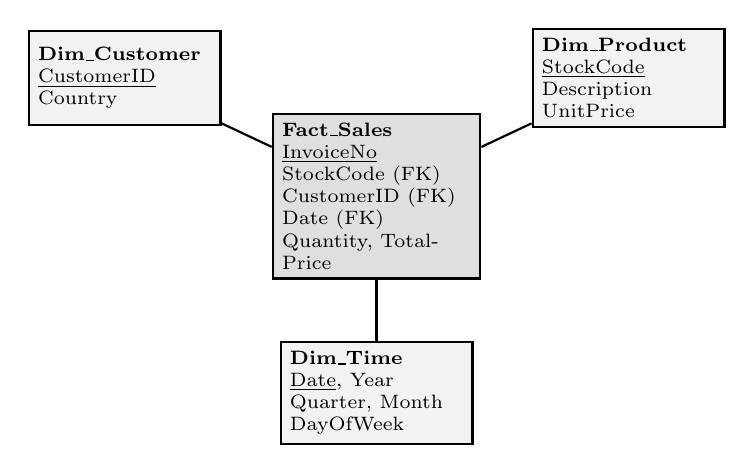
\begin{tikzpicture}[
                dim/.style={rectangle, draw, thick, text width=2.2cm, align=left, minimum height=1.2cm, fill=gray!10, font=\scriptsize},
                fact/.style={rectangle, draw, thick, text width=2.4cm, align=left, minimum height=1.6cm, fill=gray!25, font=\scriptsize}
            ]
                \node[fact] (fact) at (0,0) {
                    \textbf{Fact\_Sales}\\
                    \underline{InvoiceNo}\\
                    StockCode (FK)\\
                    CustomerID (FK)\\
                    Date (FK)\\
                    Quantity, TotalPrice
                };
                
                \node[dim] (cust) at (-3.2, 1.5) {
                    \textbf{Dim\_Customer}\\
                    \underline{CustomerID}\\
                    Country
                };
                \node[dim] (prod) at (3.2, 1.5) {
                    \textbf{Dim\_Product}\\
                    \underline{StockCode}\\
                    Description\\
                    UnitPrice
                };
                \node[dim] (time) at (0, -2.5) {
                    \textbf{Dim\_Time}\\
                    \underline{Date}, Year\\
                    Quarter, Month\\
                    DayOfWeek
                };
                
                \draw[thick] (fact) -- (cust);
                \draw[thick] (fact) -- (prod);
                \draw[thick] (fact) -- (time);
            \end{tikzpicture}
            }
            \end{center}
        \end{column}
        
        \begin{column}{0.54\textwidth}
            \textbf{Star Schema:} 1 bảng fact trung tâm kết nối các bảng dimension.

            \vspace{0.15cm}
            \textbf{VD:} \textit{``Doanh thu Q4 theo quốc gia''}\\
            $\Rightarrow$ JOIN Fact $\bowtie$ Dim\_Time $\bowtie$ Dim\_Customer.

            \vspace{0.15cm}
            \textbf{Bảng phân tích bổ sung:}
            \begin{itemize}
                \item \texttt{Customer\_RFM}: R, F, M mỗi KH
                \item \texttt{Customer\_Cluster}: RFM + cluster label phục vụ dashboard
            \end{itemize}
            
            \vspace{0.1cm}
            \footnotesize\textbf{Sau ETL:} 4,338 KH $\cdot$ 3,665 SP $\cdot$ 18,532 HĐ $\cdot$ 37 QG
        \end{column}
    \end{columns}
\end{frame}

% ==========================================
% SECTION 4: K-MEANS CLUSTERING
% ==========================================
\section{K-Means Clustering}

\begin{frame}{8. K-Means: Lý thuyết}
    \small
    \begin{columns}[T]
        \begin{column}{0.52\textwidth}
            \textbf{K-Means:} Phân cụm không giám sát, tối thiểu hóa:
            $$J = \sum_{i=1}^{k} \sum_{x \in C_i} \|x - \mu_i\|^2$$
            
            \textbf{Quy trình:}
            \begin{enumerate}
                \item Khởi tạo $k$ tâm cụm $\mu_1, \ldots, \mu_k$.
                \item \textbf{Gán:} Mỗi $x$ $\to$ cụm có $\mu_i$ gần nhất.
                \item \textbf{Cập nhật:} $\mu_i = \frac{1}{|C_i|}\sum_{x \in C_i} x$.
                \item Lặp 2--3 cho đến hội tụ.
            \end{enumerate}
            
            \footnotesize
            \textit{VD: 3 KH có RFM = (5,10,2000), (200,1,50), (3,15,5000) $\Rightarrow$ KH 1\&3 gần nhau (``Active''), KH 2 riêng (``At Risk'').}
        \end{column}
        
        \begin{column}{0.44\textwidth}
            \textbf{Chọn $k$ tối ưu:}
            \begin{itemize}
                \item \textbf{Elbow:} Vẽ Inertia theo $k$, chọn ``khuỷu tay''.
                \item \textbf{Silhouette:} Đo tách biệt giữa các cụm.
            \end{itemize}
            
            \vspace{0.1cm}
            \begin{center}
            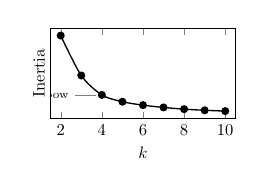
\begin{tikzpicture}[scale=0.6, every node/.style={transform shape}]
                \begin{axis}[
                    xlabel={$k$},
                    ylabel={Inertia},
                    xmin=1.5, xmax=10.5,
                    ytick=\empty,
                    xtick={2,4,6,8,10},
                    width=5.5cm,
                    height=3.5cm,
                    grid style=dashed,
                    ymajorgrids=true
                ]
                \addplot[color=black, thick, mark=*, smooth] coordinates {
                    (2,9000) (3,5500) (4,3800) (5,3200) (6,2900) (7,2700) (8,2550) (9,2450) (10,2380)
                };
                \node[pin=180:{\scriptsize Elbow}] at (axis cs:4,3800) {};
                \end{axis}
            \end{tikzpicture}
            \end{center}
            \textit{$k=4$ (elbow + domain knowledge).}
        \end{column}
    \end{columns}
\end{frame}

\begin{frame}{9. K-Means: Cấu hình \& Kết quả}
    \small
    \begin{columns}[T]
        \begin{column}{0.40\textwidth}
            \textbf{Tham số:}
            \begin{itemize}
                \item Input: RFM chuẩn hóa (4,338 KH)
                \item \texttt{n\_clusters=4, random\_state=42}
                \item \texttt{n\_init=10}
            \end{itemize}
            
            \vspace{0.15cm}
            \textbf{Metrics:}
            
            \begin{tabularx}{\linewidth}{Xr}
                \toprule
                \textbf{Metric} & \textbf{Giá trị} \\
                \midrule
                Silhouette & \textbf{0.6162} \\
                Calinski-Harabasz & 3,145.06 \\
                Davies-Bouldin & 0.7542 \\
                \bottomrule
            \end{tabularx}
            
            \vspace{0.1cm}
            \footnotesize
            \textit{Silhouette $> 0.6$: phân cụm tốt.}\\
            \textit{Davies-Bouldin $< 1$: cụm chặt.}
        \end{column}
        
        \begin{column}{0.55\textwidth}
            \textbf{Profiling 4 cụm (RFM trung bình):}
            
            \footnotesize
            \begin{tabularx}{\linewidth}{X r r r r}
                \toprule
                & \textbf{C0} & \textbf{C1} & \textbf{C2} & \textbf{C3} \\
                \midrule
                \#KH & 3,054 & 1,067 & 13 & 204 \\
                R (ngày) & 44 & 248 & 7 & 16 \\
                F (lần) & 3.7 & 1.6 & 82.5 & 22.3 \\
                M (£) & 1,354 & 479 & 127K & 12,691 \\
                \bottomrule
            \end{tabularx}
            
            \small
            \vspace{0.15cm}
            \textbf{Diễn giải:}
            \begin{itemize}
                \item \textbf{C0 -- Low Value:} Đông nhất và chi tiêu thấp.
                \item \textbf{C1 -- At Risk:} Đã inactive lâu ngày, chi tiêu thấp.
                \item \textbf{C2 -- Champions:} Tần suất cao và chi tiêu cực cao, thường xuyên (13 KH).
                \item \textbf{C3 -- Loyal:} Mua gần đây, thường xuyên, chi nhiều.
            \end{itemize}
        \end{column}
    \end{columns}
\end{frame}

% ==========================================
% SECTION 5: XGBOOST
% ==========================================
\section{XGBoost --- Dự đoán CLV}

\begin{frame}{10. XGBoost Regression: Lý thuyết}
    \small
    \begin{columns}[T]
        \begin{column}{0.52\textwidth}
            \textbf{XGBoost:} Kết hợp nhiều cây quyết định yếu thành mô hình mạnh (gradient boosting).
            
            \vspace{0.1cm}
            \textbf{Hàm mục tiêu:}
            $$\mathcal{L} = \underbrace{\sum_{i} l(y_i, \hat{y}_i)}_{\text{Loss}} + \underbrace{\sum_{k} \Omega(f_k)}_{\text{Regularization}}$$
            
            \textbf{Ý tưởng:}
            \begin{enumerate}
                \item Cây 1 dự đoán $\hat{y}^{(1)}$.
                \item Cây 2 học \textit{sai số} $y - \hat{y}^{(1)}$.
                \item Cây $t$: $\hat{y}^{(t)} = \sum_{k=1}^{t} f_k(x)$.
            \end{enumerate}

            \footnotesize
            \textit{VD: Cây 1 dự đoán £1000, thực tế £1500 $\Rightarrow$ cây 2 học chênh lệch £500.}
        \end{column}
        
        \begin{column}{0.44\textwidth}
            \begin{center}
            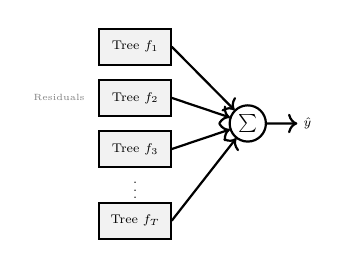
\begin{tikzpicture}[scale=0.65, every node/.style={transform shape},
                tree/.style={rectangle, draw, thick, fill=gray!10, minimum width=1.4cm, minimum height=0.7cm, align=center, font=\scriptsize},
                sum/.style={circle, draw, thick, inner sep=2pt}
            ]
                \node[tree] (t1) at (0,2.5) {Tree $f_1$};
                \node[tree] (t2) at (0,1.5) {Tree $f_2$};
                \node[tree] (t3) at (0,0.5) {Tree $f_3$};
                \node[font=\scriptsize] at (0,-0.2) {$\vdots$};
                \node[tree] (tn) at (0,-0.9) {Tree $f_T$};
                
                \node[sum] (plus) at (2.2,1) {$\sum$};
                \node[right=0.6cm of plus, font=\scriptsize] (pred) {$\hat{y}$};
                
                \draw[->, thick] (t1.east) -- (plus);
                \draw[->, thick] (t2.east) -- (plus);
                \draw[->, thick] (t3.east) -- (plus);
                \draw[->, thick] (tn.east) -- (plus);
                \draw[->, thick] (plus) -- (pred);
                
                \node[font=\tiny, gray, left=0.15cm of t2] {Residuals};
            \end{tikzpicture}
            \end{center}
            
            \vspace{0.1cm}
            \textbf{Regularization} $\Omega(f_k)$: Penalize cây quá phức tạp $\Rightarrow$ chống overfitting.
        \end{column}
    \end{columns}
\end{frame}

\begin{frame}{11. XGBoost CLV: Cấu hình \& Kết quả}
    \small
    \begin{columns}[T]
        \begin{column}{0.45\textwidth}
            \textbf{Bài toán:} Dự đoán \textit{FutureSpend} (tổng chi tiêu 3 tháng cuối) từ RFM.
            
            \vspace{0.15cm}
            \textbf{Tham số:}
            \begin{itemize}
                \item Train/Test: 80/20
                \item \texttt{n\_estimators=100}
                \item \texttt{learning\_rate=0.1}
                \item \texttt{max\_depth=5}
            \end{itemize}
            
            \vspace{0.15cm}
            \textbf{Feature Importance:}
            
            \begin{tabularx}{\linewidth}{Xr}
                \toprule
                \textbf{Feature} & \textbf{Importance} \\
                \midrule
                Monetary & \textbf{0.4546} \\
                Recency & 0.3497 \\
                Frequency & 0.1957 \\
                \bottomrule
            \end{tabularx}
        \end{column}
        
        \begin{column}{0.5\textwidth}
            \textbf{Metrics:}
            
            \begin{tabularx}{\linewidth}{Xr}
                \toprule
                \textbf{Metric} & \textbf{Giá trị} \\
                \midrule
                RMSE & 4,753.40 \\
                MAE & 764.49 \\
                Median AE & 240.13 \\
                R² & 0.3832 \\
                Explained Var. & 0.3833 \\
                sMAPE & 124.89\% \\
                \bottomrule
            \end{tabularx}
            
            \vspace{0.15cm}
            \textbf{Phân tích:}
            \begin{itemize}
                \item R²=0.38: Giải thích 38\% biến thiên.
                \item MedAE (240) $\ll$ MAE (764): có outlier.
                \item \textbf{Monetary} mạnh nhất --- ``chi nhiều $\Rightarrow$ tiếp tục chi nhiều''.
            \end{itemize}
        \end{column}
    \end{columns}
\end{frame}

% ==========================================
% SECTION 6: FP-GROWTH
% ==========================================
\section{FP-Growth --- Luật kết hợp}

\begin{frame}{12. FP-Growth: Lý thuyết}
    \small
    \begin{columns}[T]
        \begin{column}{0.52\textwidth}
            \textbf{FP-Growth:} Khai phá tập phổ biến bằng FP-Tree nén --- \textbf{không sinh ứng viên} như Apriori.
            
            \vspace{0.15cm}
            \textbf{3 metrics:}
            \begin{itemize}
                \item \textbf{Support:} $P(A \cup B)$\\
                    \textit{VD: 150/10K GD chứa Mug \& Plate $\Rightarrow$ 0.015.}
                \item \textbf{Confidence:} $P(B|A) = \frac{P(A \cup B)}{P(A)}$\\
                    \textit{VD: 150/300 $\Rightarrow$ Conf = 0.5.}
                \item \textbf{Lift:} $\frac{P(B|A)}{P(B)}$, Lift $> 1$ = tương quan dương.\\
                    \textit{VD: Lift=10 $\Rightarrow$ mua Mug tăng XS mua Plate gấp 10$\times$.}
            \end{itemize}
        \end{column}
        
        \begin{column}{0.44\textwidth}
            \begin{center}
            \begin{tikzpicture}[scale=0.65, every node/.style={transform shape}]
                \node[draw, circle, thick, fill=gray!10] (root) at (0,2.5) {\tiny null};
                \node[draw, circle, thick, fill=gray!10] (a) at (-0.8,1.5) {\tiny A:3};
                \node[draw, circle, thick, fill=gray!10] (b1) at (-0.8,0.5) {\tiny B:2};
                \node[draw, circle, thick, fill=gray!10] (b2) at (0.8,1.5) {\tiny B:1};
                \node[draw, circle, thick, fill=gray!10] (c) at (-0.8,-0.4) {\tiny C:1};
                
                \draw[thick] (root) -- (a);
                \draw[thick] (a) -- (b1);
                \draw[thick] (b1) -- (c);
                \draw[thick] (root) -- (b2);
                
                \node[font=\scriptsize, gray] at (0,-1.1) {FP-Tree nén giao dịch};
            \end{tikzpicture}
            \end{center}
            
            \vspace{0.1cm}
            \textbf{Ưu điểm FP-Growth:}
            \begin{itemize}
                \item Quét DB \textbf{2 lần} (vs Apriori: $k$ lần)
                \item Không sinh candidate set
                \item Nhanh hơn với dữ liệu lớn
            \end{itemize}
        \end{column}
    \end{columns}
\end{frame}

\begin{frame}{13. FP-Growth: Cấu hình \& Kết quả}
    \small
    \begin{columns}[T]
        \begin{column}{0.45\textwidth}
            \textbf{Tham số:}
            \begin{itemize}
                \item Basket matrix: giao dịch UK, one-hot
                \item \texttt{min\_support = 0.015} (1.5\%)
                \item Luật: \texttt{lift $\geq$ 1.5}
            \end{itemize}
            
            \vspace{0.15cm}
            \textbf{Kết quả:}
            
            \begin{tabularx}{\linewidth}{Xr}
                \toprule
                \textbf{Metric} & \textbf{Giá trị} \\
                \midrule
                Frequent itemsets & \textbf{440} \\
                Rules generated & \textbf{214} \\
                Avg support & 0.0191 \\
                Avg confidence & 0.4375 \\
                Avg lift & 10.199 \\
                Max lift & 28.628 \\
                \bottomrule
            \end{tabularx}
        \end{column}
        
        \begin{column}{0.5\textwidth}
            \textbf{Phân tích:}
            \begin{itemize}
                \item 214 luật: đủ cho recommendation.
                \item Avg lift = 10.2: tương quan mạnh.
                \item Max lift = 28.6: cặp SP cực mạnh.
                \item Pattern: \textit{support thấp, lift cao} $\Rightarrow$ phù hợp gợi ý cá nhân hóa.
            \end{itemize}
            
            \vspace{0.15cm}
            \textbf{VD luật:}\\
            \footnotesize
            \textit{Mua `ALARM CLOCK RED' $\Rightarrow$ xác suất cao mua `ALARM CLOCK GREEN'}\\
            $\Rightarrow$ Gợi ý bundle cùng dòng sản phẩm.
        \end{column}
    \end{columns}
\end{frame}

\begin{frame}{Kiểm thử mô hình và recommendation}
    \small
    \begin{itemize}
        \item \textbf{KMeans:} 3 probe profiles mới được dùng để kiểm tra khả năng gán cụm của mô hình.
        \item \textbf{XGBoost:} 5 mẫu holdout được ghi lại với actual/predicted để kiểm tra trên dữ liệu chưa thấy.
        \item \textbf{FP-Growth:} Top rules và một ví dụ khách hàng cụ thể được dùng để minh họa recommendation bán chéo.
        \item Toàn bộ bảng chi tiết được sinh tự động trong \texttt{generated/metrics.tex}.
    \end{itemize}
\end{frame}

% ==========================================
% SECTION 7: EXPERIMENT RESULTS
% ==========================================
\section{Kết quả thực nghiệm}

\begin{frame}{14. Tổng hợp Pipeline Data Profile}
    \small
    \begin{columns}[T]
        \begin{column}{0.42\textwidth}
            \textbf{Thống kê dữ liệu:}
            
            \begin{tabularx}{\linewidth}{Xr}
                \toprule
                \textbf{Metric} & \textbf{Value} \\
                \midrule
                Raw rows & 541,909 \\
                After dedup & 536,641 \\
                Clean rows & 392,692 \\
                Customers & 4,338 \\
                Products & 3,665 \\
                Invoices & 18,532 \\
                Countries & 37 \\
                Revenue & £8,887,209 \\
                \bottomrule
            \end{tabularx}
        \end{column}
        
        \begin{column}{0.54\textwidth}
            \textbf{Đánh giá định lượng:}
            
            \footnotesize
            \begin{tabularx}{\linewidth}{llX}
                \toprule
                \textbf{Mô hình} & \textbf{Metric chính} & \textbf{Đánh giá} \\
                \midrule
                KMeans & Silhouette = 0.62 & \textbf{Đạt} \\
                & DB = 0.75 & \\
                \midrule
                XGBoost & R² = 0.38 & \textbf{Đạt} \\
                & MAE = 764 & \textbf{một phần} \\
                \midrule
                FP-Growth & 214 rules & \textbf{Đạt} \\
                & Avg lift = 10.2 & \\
                \bottomrule
            \end{tabularx}
            
            \small
            \vspace{0.15cm}
            \textit{Pipeline sinh: 17 figures, summary.json, metrics.tex, 4 model .pkl.}
        \end{column}
    \end{columns}
\end{frame}

\begin{frame}{Trực quan: K-Means Clustering}
    \begin{columns}[c]
        \begin{column}{0.48\textwidth}
            \begin{figure}
                \centering
                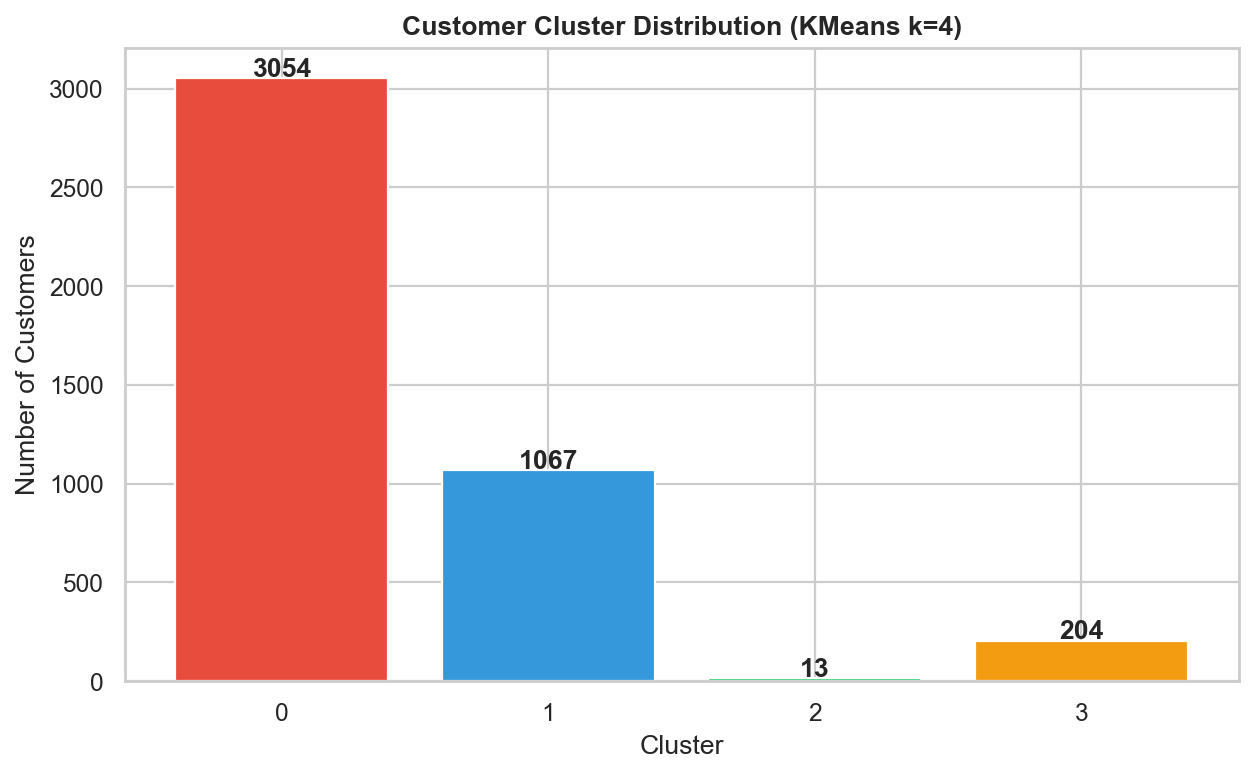
\includegraphics[width=0.9\linewidth]{../report/generated/figures/cluster_distribution.png}
                \caption*{\scriptsize Phân bố KH theo cụm ($k=4$)}
            \end{figure}
        \end{column}
        \begin{column}{0.48\textwidth}
            \begin{figure}
                \centering
                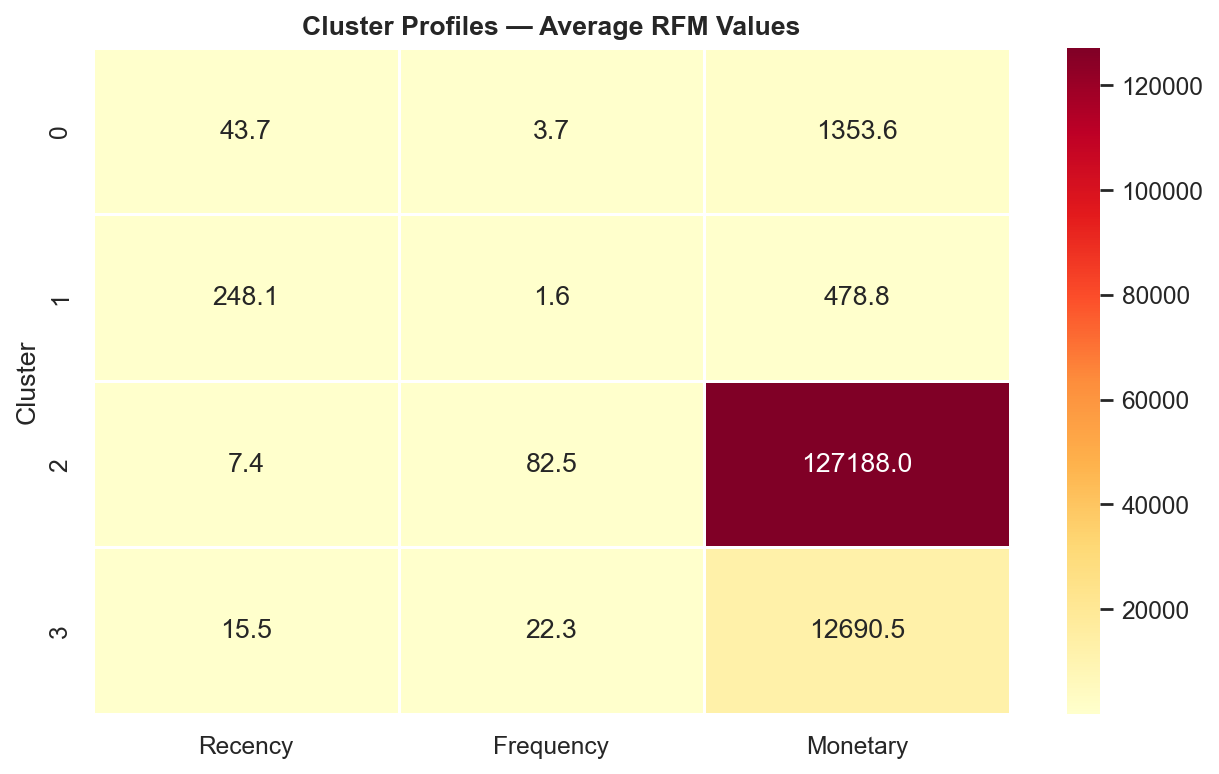
\includegraphics[width=0.9\linewidth]{../report/generated/figures/cluster_heatmap.png}
                \caption*{\scriptsize Heatmap RFM trung bình mỗi cụm}
            \end{figure}
        \end{column}
    \end{columns}
    \footnotesize
    \textbf{Nhận xét:} C0 (Loyal) chiếm đa số (3,054 KH). C2 (Champions) chỉ 13 KH nhưng M = £127K.
\end{frame}

\begin{frame}{Trực quan: Elbow + Silhouette \& 3D Scatter}
    \begin{columns}[c]
        \begin{column}{0.48\textwidth}
            \begin{figure}
                \centering
                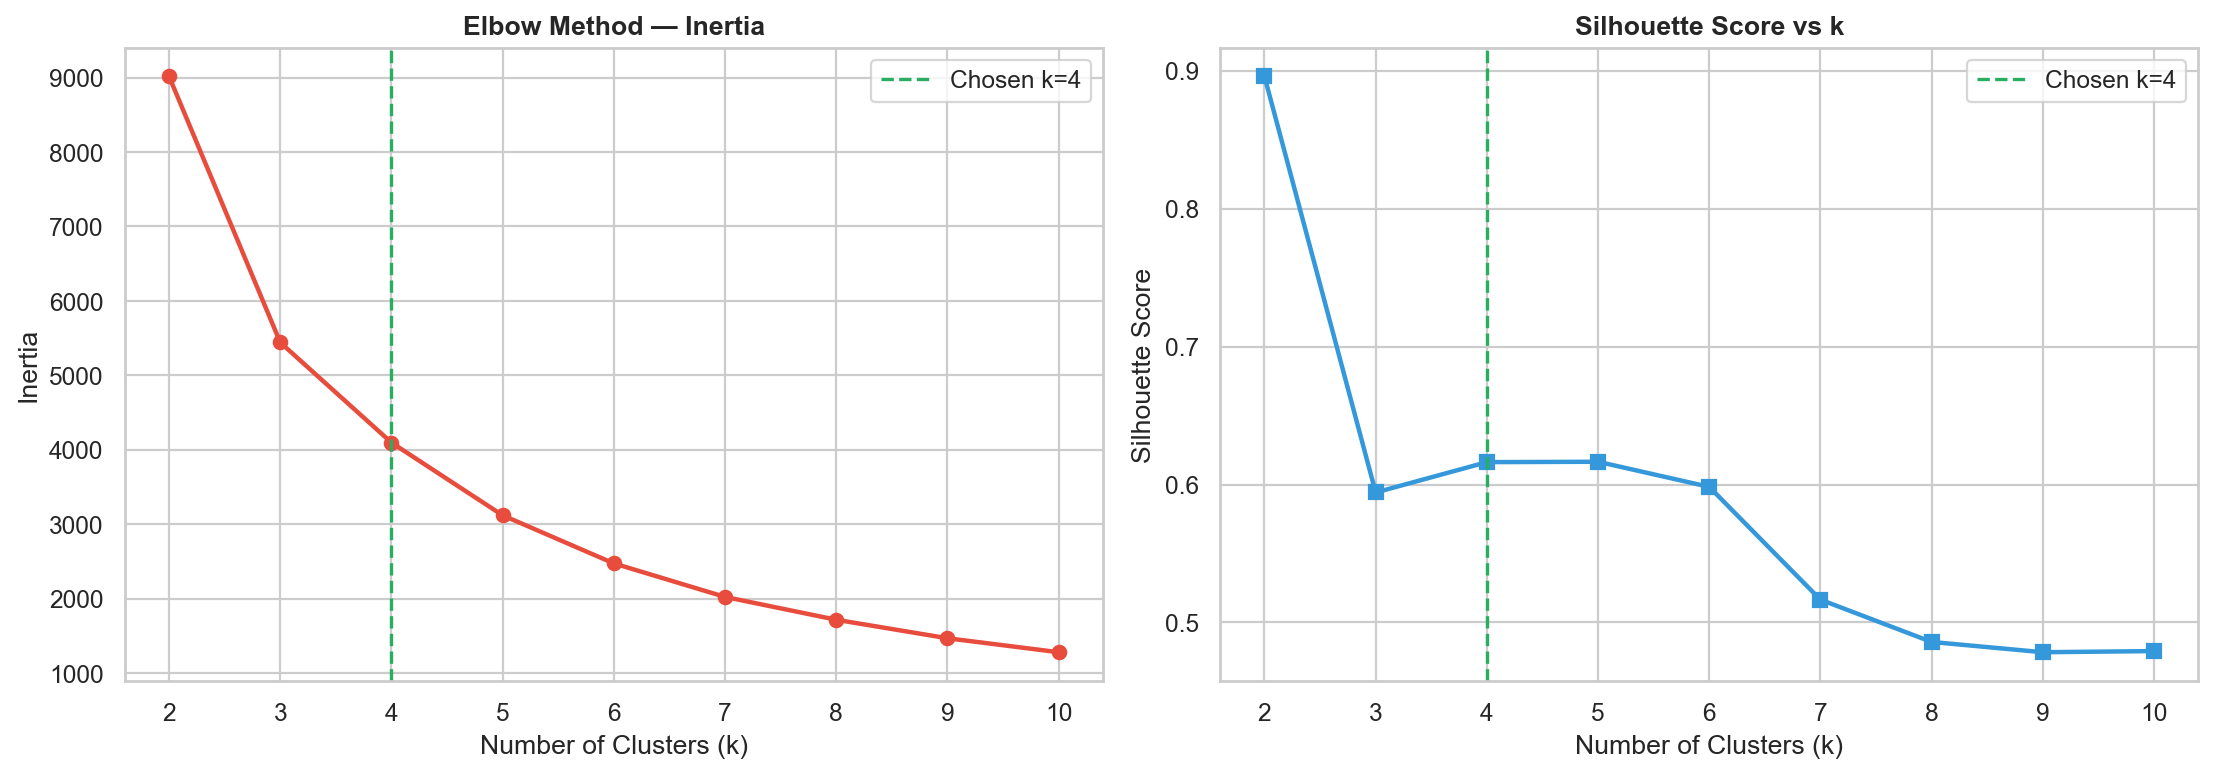
\includegraphics[width=0.75\linewidth]{../report/generated/figures/elbow_silhouette.png}
                \caption*{\scriptsize Elbow Method \& Silhouette Score}
            \end{figure}
        \end{column}
        \begin{column}{0.48\textwidth}
            \begin{figure}
                \centering
                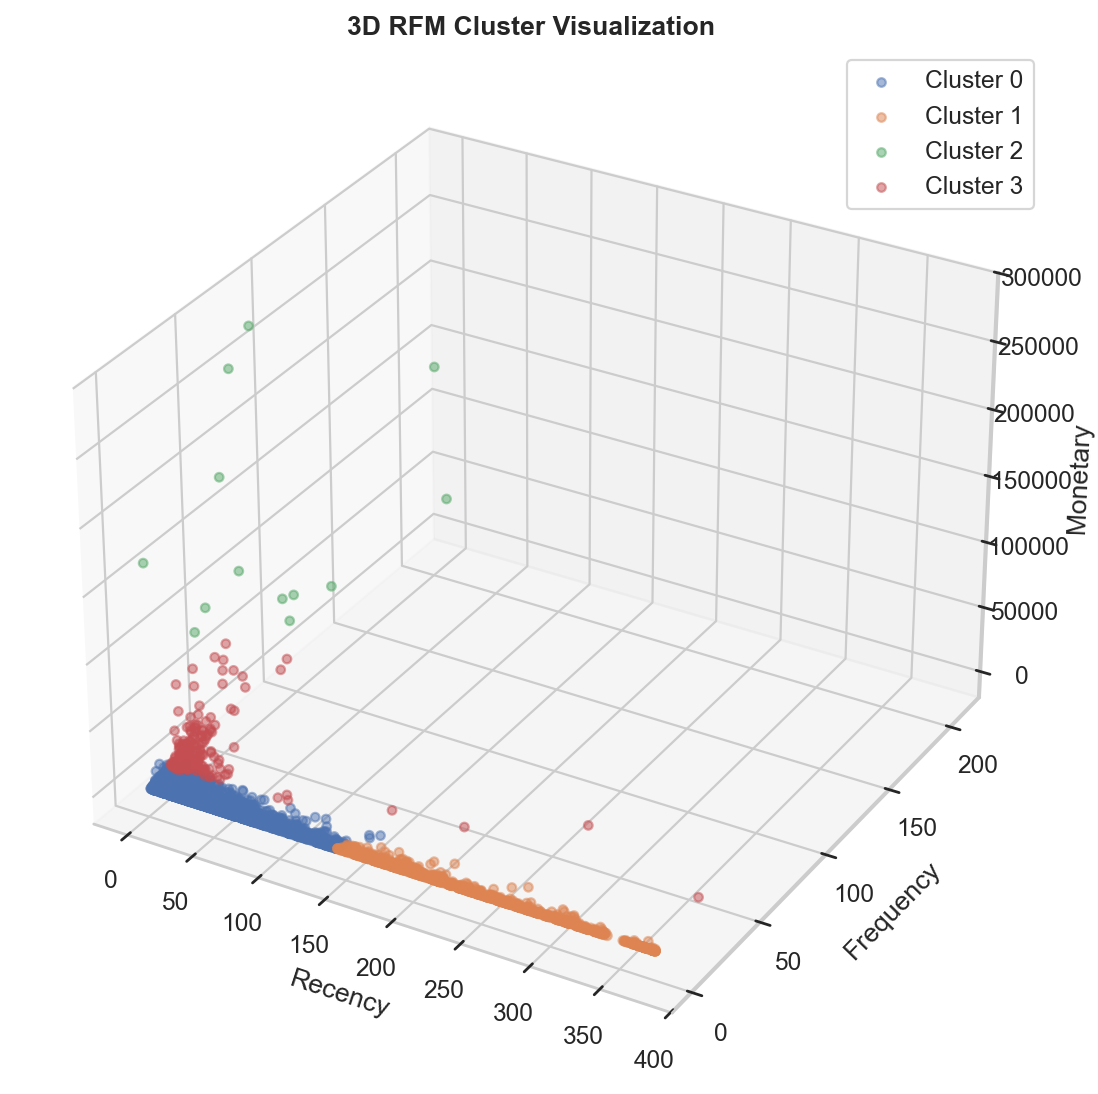
\includegraphics[width=0.75\linewidth]{../report/generated/figures/cluster_3d.png}
                \caption*{\scriptsize 3D scatter: cụm KH trong không gian RFM}
            \end{figure}
        \end{column}
    \end{columns}
    \footnotesize
    \textbf{Nhận xét:} Elbow rõ tại $k=4$. Silhouette cao nhất tại $k=2$ nhưng $k=4$ chi tiết hơn.
\end{frame}

\begin{frame}{Trực quan: XGBoost CLV Prediction}
    \begin{columns}[c]
        \begin{column}{0.48\textwidth}
            \begin{figure}
                \centering
                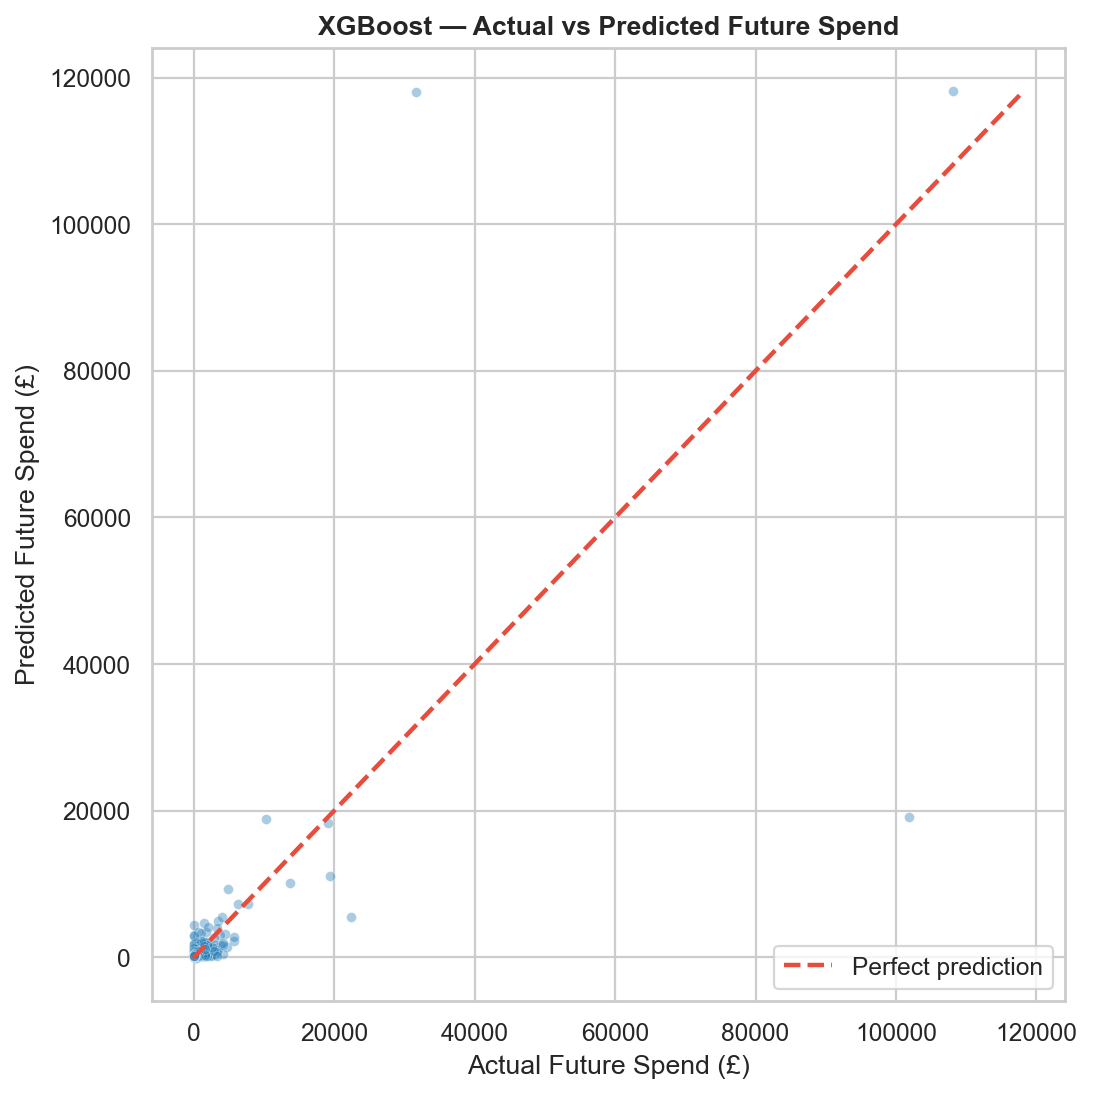
\includegraphics[width=0.75\linewidth]{../report/generated/figures/xgb_actual_vs_predicted.png}
                \caption*{\scriptsize Actual vs Predicted}
            \end{figure}
        \end{column}
        \begin{column}{0.48\textwidth}
            \begin{figure}
                \centering
                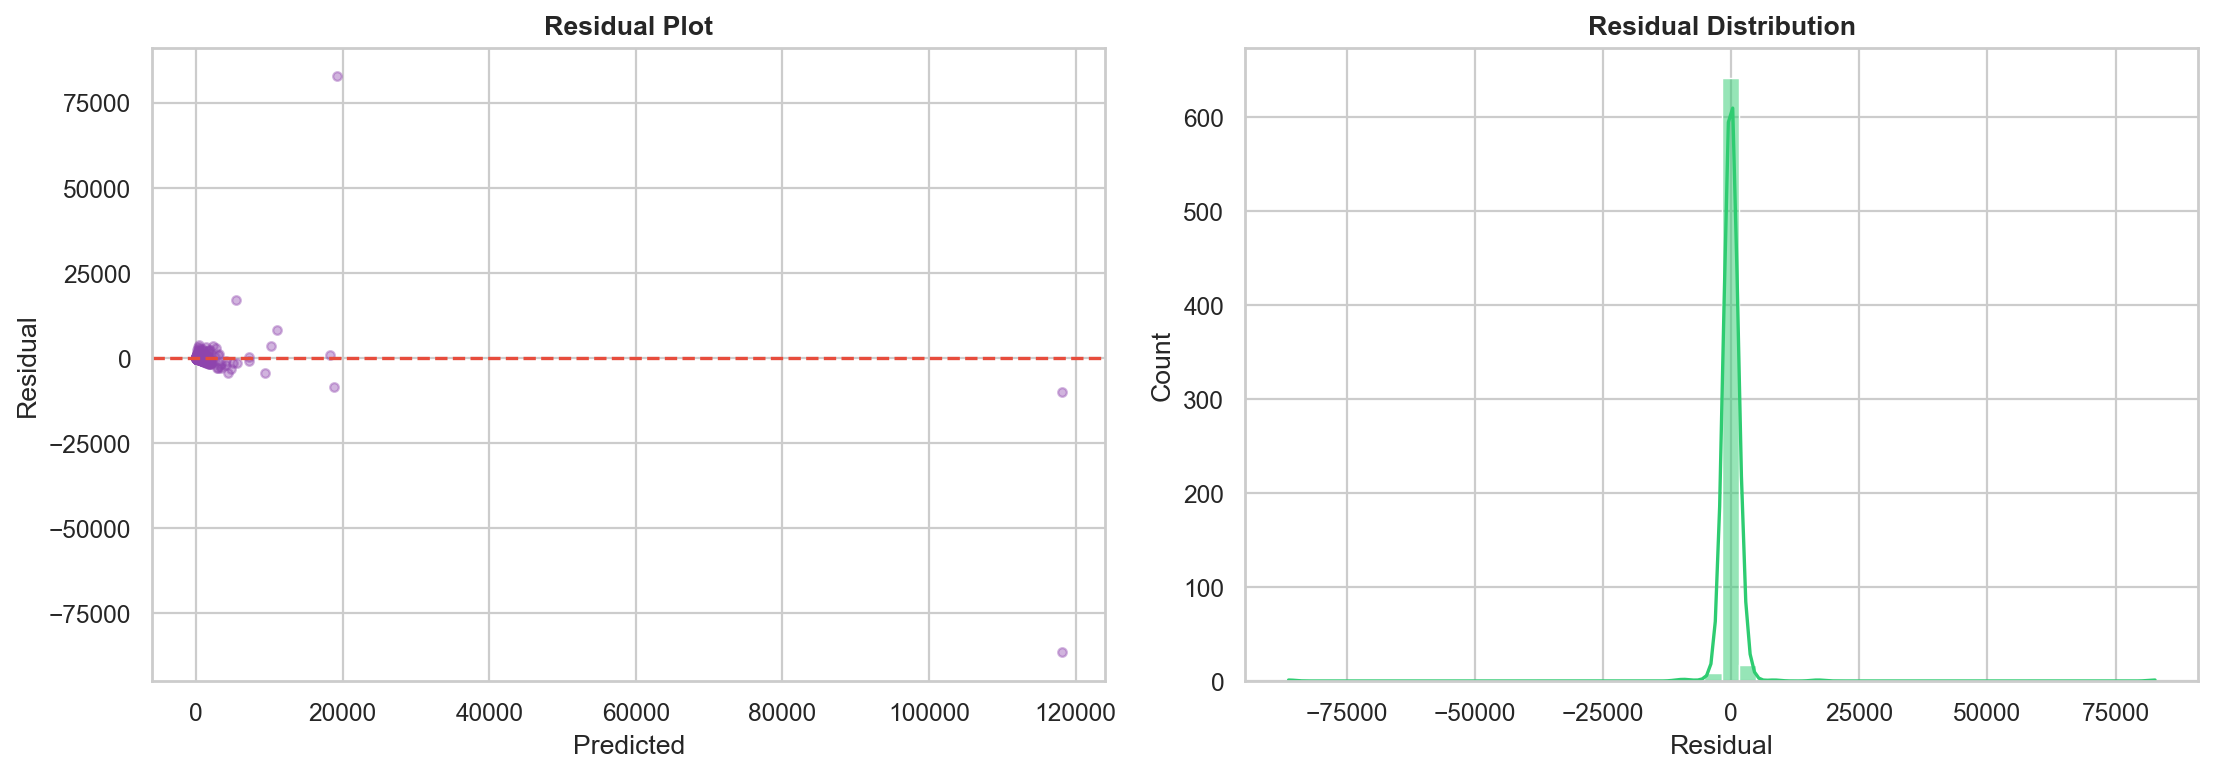
\includegraphics[width=0.75\linewidth]{../report/generated/figures/xgb_residuals.png}
                \caption*{\scriptsize Residual analysis}
            \end{figure}
        \end{column}
    \end{columns}
    \footnotesize
    \textbf{Nhận xét:} Điểm gần $y=x$ $\Rightarrow$ dự đoán hợp lý. Residual lệch phải $\Rightarrow$ underestimate outlier.
\end{frame}

\begin{frame}{Trực quan: Feature Importance \& FP-Growth}
    \begin{columns}[c]
        \begin{column}{0.48\textwidth}
            \begin{figure}
                \centering
                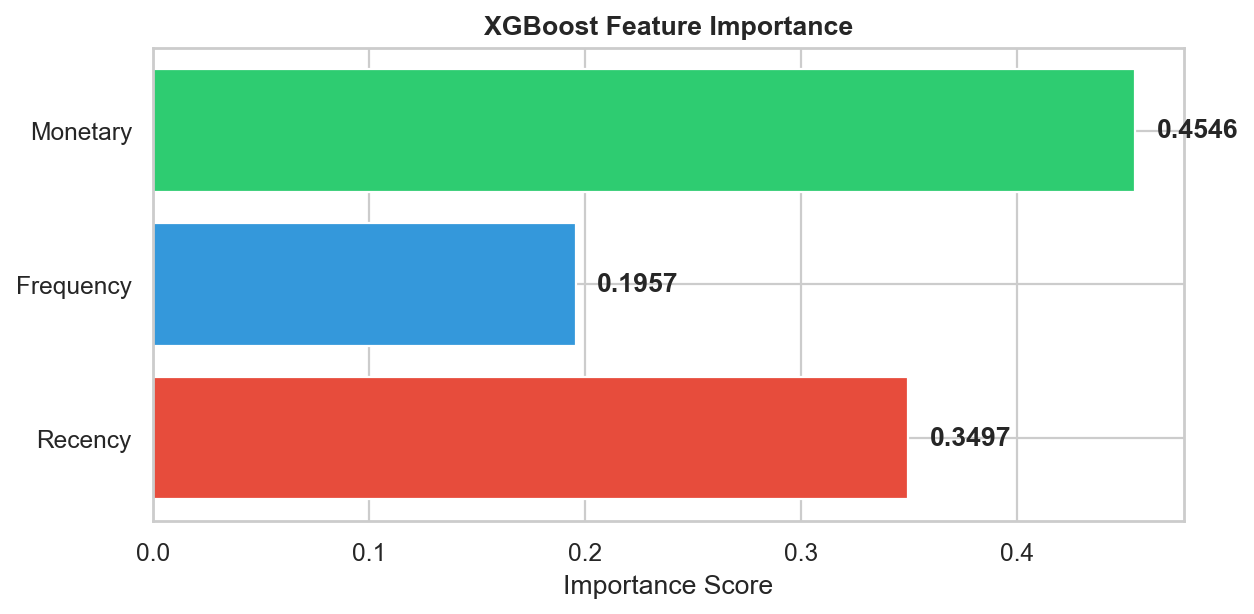
\includegraphics[width=0.85\linewidth]{../report/generated/figures/feature_importance.png}
                \caption*{\scriptsize Feature Importance (XGBoost)}
            \end{figure}
        \end{column}
        \begin{column}{0.48\textwidth}
            \begin{figure}
                \centering
                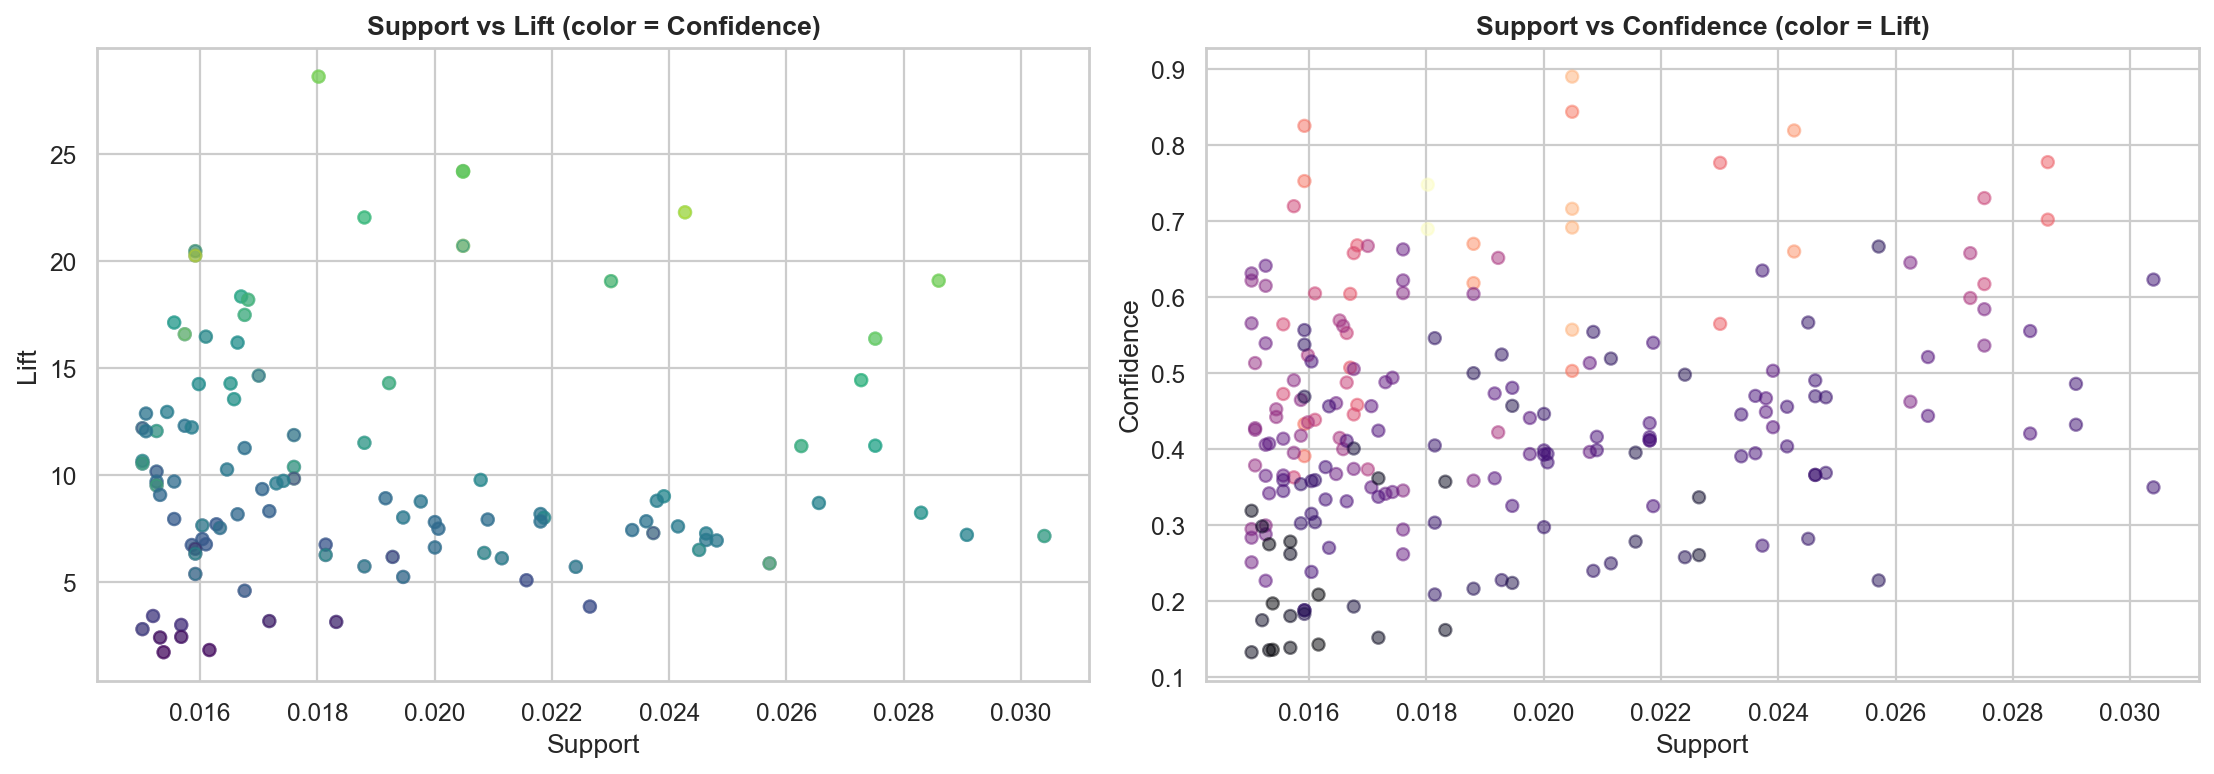
\includegraphics[width=0.9\linewidth]{../report/generated/figures/rules_support_lift.png}
                \caption*{\scriptsize Support vs Lift \& Confidence}
            \end{figure}
        \end{column}
    \end{columns}
    \footnotesize
    \textbf{Nhận xét:} Monetary = 45.5\% importance. FP-Growth: lift cao ($>$10) + support thấp --- gợi ý cá nhân hóa.
\end{frame}

\begin{frame}[fragile]{Trực quan: Holdout Test \& Probe Predictions}
    \textbf{XGBoost Holdout Test Examples (5 Test Instances)}
    \vspace{-0.15cm}
    \begin{center}
        \tiny
        \setlength{\tabcolsep}{3pt}
        \renewcommand{\arraystretch}{1.15}
        \begin{tabular}{rrrrrr}
        \toprule
        \textbf{Recency} & \textbf{Frequency} & \textbf{Monetary} & \textbf{Actual} & \textbf{Predicted} & \textbf{Error} \\
        \midrule
        15.00 & 3.00 & 855.00 & 1763.23 & 553.38 & -1209.85 \\
        24.00 & 3.00 & 539.13 & 213.64 & 313.28 & 99.64 \\
        15.00 & 5.00 & 797.02 & 219.12 & 553.38 & 334.26 \\
        91.00 & 2.00 & 1399.11 & 591.90 & 629.75 & 37.85 \\
        233.00 & 1.00 & 63.00 & 0.00 & 38.84 & 38.84 \\
        \bottomrule
        \end{tabular}
    \end{center}
    
    \vspace{0.1cm}
    \textbf{KMeans Probe Predictions on New Customer Profiles}
    \vspace{-0.15cm}
    \begin{center}
        \tiny
        \setlength{\tabcolsep}{5pt}
        \renewcommand{\arraystretch}{1.15}
        \begin{tabular}{lrrrr}
        \toprule
        \textbf{Profile} & \textbf{Recency} & \textbf{Frequency} & \textbf{Monetary} & \textbf{Cluster} \\
        \midrule
        at\_risk & 263.00 & 1.00 & 155.30 & 1 \\
        loyal & 51.00 & 9.00 & 668.57 & 0 \\
        champion & 5.00 & 9.00 & 3640.84 & 0 \\
        \bottomrule
        \end{tabular}
    \end{center}
    
    \vspace{0.15cm}
    \small
    \textbf{Nhận xét:} XGBoost: 4/5 dự đoán hợp lý, lỗi lớn nhất do outlier. KMeans: cả 3 probe được gán tương đối đúng cụm (at\_risk=1, loyal/champion=0).
\end{frame}

\begin{frame}[fragile]{Trực quan: FP-Growth Top Rules \& Customer Recommendation}
    
    \textbf{Top 5 Association Rules by Lift}
    
    \vspace{-0.15cm}
    \begin{center}
        \scriptsize
        \setlength{\tabcolsep}{2.5pt}
        \renewcommand{\arraystretch}{1.1}
        \begin{tabular}{>{\raggedright\arraybackslash}p{2.9cm}>{\raggedright\arraybackslash}p{2.9cm}rrr}
        \toprule
        \textbf{Antecedents} & \textbf{Consequents} & \textbf{Supp.} & \textbf{Conf.} & \textbf{Lift} \\
        \midrule
        WOODEN HEART XMAS & WOODEN STAR XMAS & 0.0180 & 0.6897 & 28.63 \\
        WOODEN STAR XMAS & WOODEN HEART XMAS & 0.0180 & 0.7481 & 28.63 \\
        GREEN REGENCY TEA & PINK\&ROSES REGENCY TEA & 0.0205 & 0.5572 & 24.22 \\
        PINK\&ROSES REGENCY TEA & GREEN REGENCY TEA & 0.0205 & 0.8903 & 24.22 \\
        PINK REGENCY TEA & GREEN\&ROSES REGENCY TEA & 0.0205 & 0.6917 & 24.19 \\
        \bottomrule
        \end{tabular}
    \end{center}
    
    \textbf{Nhận xét:} Những mặt hàng cùng loại (cùng dòng sản phẩm) có lift rất cao ($>$24) $\Rightarrow$ cơ hội cross-sell mạnh.
\end{frame}

\begin{frame}[fragile]{Trực quan: FP-Growth Top Rules \& Customer Recommendation}

    \textbf{Customer Recommendation Example}
    
    \vspace{-0.15cm}
    \begin{center}
        \scriptsize
        \setlength{\tabcolsep}{4pt}
        \renewcommand{\arraystretch}{1.15}
        \begin{tabular}{>{\raggedright\arraybackslash}p{3.2cm}>{\raggedright\arraybackslash}p{5.2cm}}
        \toprule
        \textbf{Field} & \textbf{Value} \\
        \midrule
        CustomerID & 12886 \\
        Purchased Items & 12 PENCILS TUBE WOODLAND, 3 HOOK PHOTO SHELF, BISCUIT CUTTERS SET, [\ldots +7 more] \\
        Matched Rules & PINK \& ROSES REGENCY TEA \\
        \textbf{Recommended} & \textbf{GREEN REGENCY TEA} \\
        Support & 0.0205 \\
        Confidence & 0.8903 \\
        Lift & 24.2167 \\
        \bottomrule
        \end{tabular}
    \end{center}
    
    \vspace{0.1cm}
    \small
    \textbf{Nhận xét:} KH 12886 đã mua PINK + ROSES $\Rightarrow$ gợi ý GREEN với confidence=89\%.
\end{frame}

\begin{frame}{Trực quan: Business Insights}
    \begin{columns}[c]
        \begin{column}{0.48\textwidth}
            \begin{figure}
                \centering
                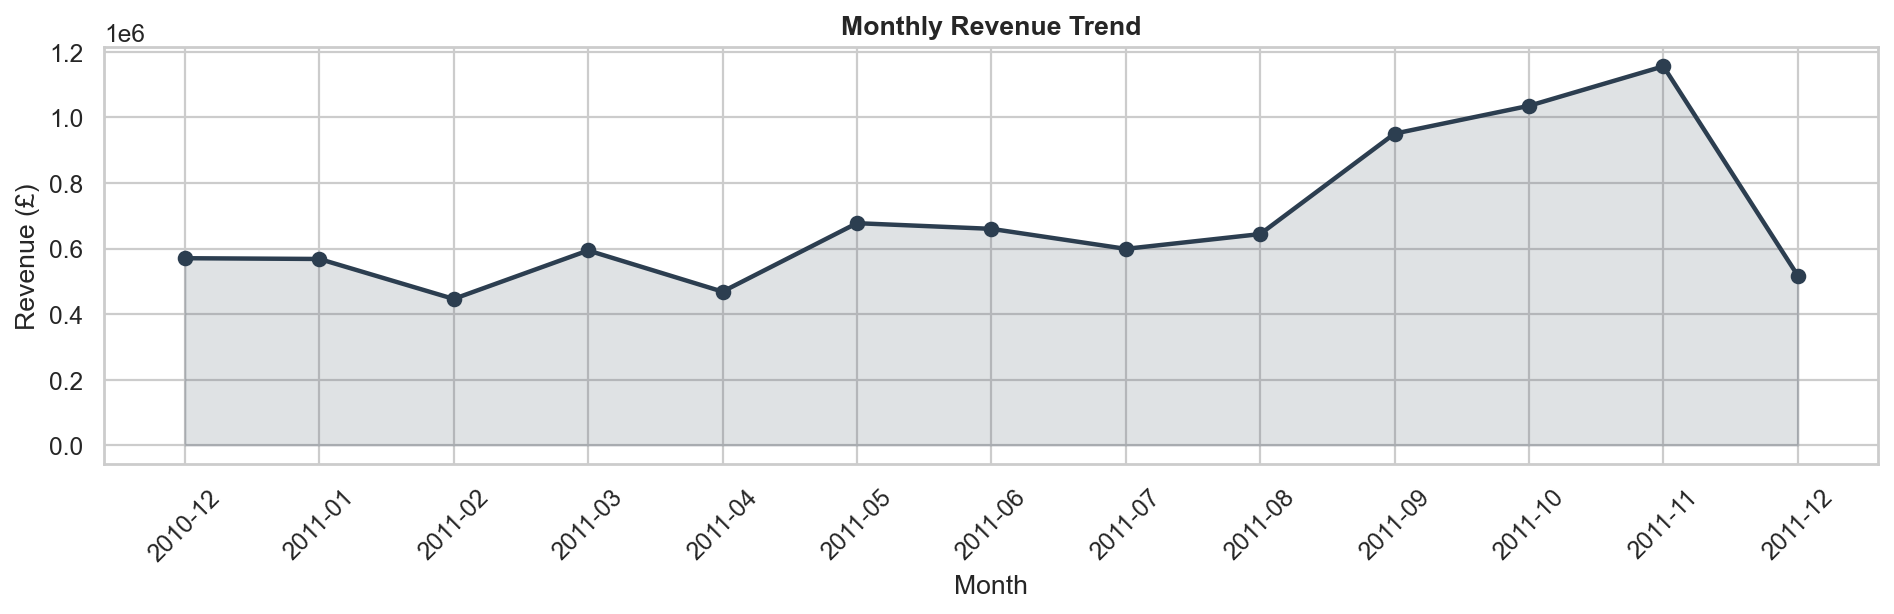
\includegraphics[width=0.9\linewidth]{../report/generated/figures/monthly_revenue.png}
                \caption*{\scriptsize Doanh thu theo tháng}
            \end{figure}
        \end{column}
        \begin{column}{0.48\textwidth}
            \begin{figure}
                \centering
                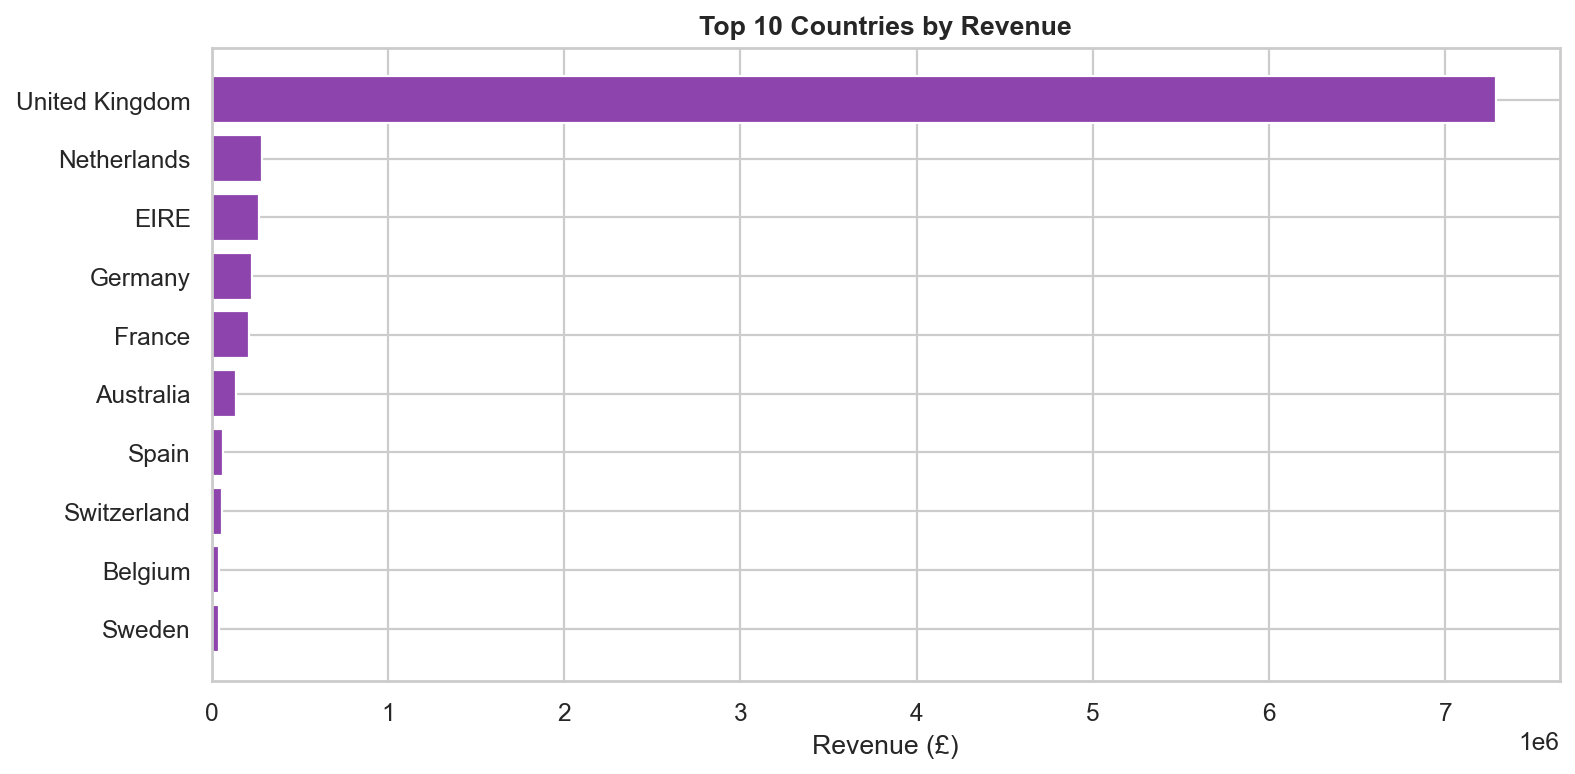
\includegraphics[width=0.9\linewidth]{../report/generated/figures/top_countries.png}
                \caption*{\scriptsize Top 10 quốc gia theo doanh thu}
            \end{figure}
        \end{column}
    \end{columns}
    
    \footnotesize
    \textbf{Insights:}
    \begin{itemize}
        \item Doanh thu tăng mạnh Q4 (mùa lễ) $\Rightarrow$ tăng inventory trước Q4.
        \item UK chiếm ưu thế $\Rightarrow$ cơ hội mở rộng sang EU.
    \end{itemize}
\end{frame}

% ==========================================
% SECTION 8: APPLICATION
% ==========================================
\section{Ứng dụng \& Dashboard}

\begin{frame}{15. Ứng dụng --- Decision Support}
    \small
    \begin{columns}[T]
        \begin{column}{0.5\textwidth}
            \textbf{Dashboard (Streamlit + Plotly):} 3 tab:
            \begin{enumerate}
                \item \textbf{Dashboard:} KPI + 6+ biểu đồ tương tác.
                \item \textbf{AI Customer Intelligence:} Nhập CustomerID $\to$ phân cụm, CLV, cross-sell.
                \item \textbf{Pipeline Log:} Nhật ký ETL + training.
            \end{enumerate}
        \end{column}
        
        \begin{column}{0.46\textwidth}
            \footnotesize
            \begin{tabularx}{\linewidth}{lX}
                \toprule
                \textbf{Mô hình} & \textbf{Hành động KD} \\
                \midrule
                KMeans & Khuyến mãi cho At Risk, loyalty cho Champions \\
                \midrule
                XGBoost & Đầu tư budget vào KH CLV cao \\
                \midrule
                FP-Growth & Cross-sell \& bundling trên web/email \\
                \bottomrule
            \end{tabularx}
            
            \small
            \vspace{0.15cm}
            \textbf{VD:} KH 14911 (Champions) $\Rightarrow$ CLV = £15,200 $\Rightarrow$ gợi ý bundle sản phẩm.
        \end{column}
    \end{columns}
\end{frame}

% ==========================================
% SECTION 9: CONCLUSION
% ==========================================
\section{Kết luận}

\begin{frame}{16. Đánh giá mục tiêu \& Giới hạn}
    \small
    \begin{columns}[T]
        \begin{column}{0.48\textwidth}
            \textbf{Đánh giá mục tiêu:}
            \begin{itemize}
                \item[\checkmark] \textbf{ETL:} Tự động, reproducible.
                \item[\checkmark] \textbf{Star Schema:} 3 Dim + 1 Fact + 2 bảng phân tích.
                \item[\checkmark] \textbf{K-Means:} 4 cụm (Sil=0.62).
                \item[$\sim$] \textbf{XGBoost:} R²=0.38, cần cải thiện.
                \item[\checkmark] \textbf{FP-Growth:} 214 luật, lift cao.
                \item[\checkmark] \textbf{Dashboard:} Tương tác, AI tích hợp.
            \end{itemize}
        \end{column}
        
        \begin{column}{0.48\textwidth}
            \textbf{Giới hạn:}
            \begin{itemize}
                \item Dữ liệu chỉ $\sim$1 năm, thiếu biến bổ sung.
                \item K-Means: giả định cụm cầu, nhạy outlier.
                \item XGBoost: chưa tuning hệ thống.
                \item FP-Growth: chỉ cho thị trường UK.
                \item Dashboard: chưa authentication, chưa cloud.
            \end{itemize}
        \end{column}
    \end{columns}
\end{frame}

\begin{frame}{17. Hướng phát triển tương lai}
    \small
    \begin{columns}[T]
        \begin{column}{0.48\textwidth}
            \textbf{Cải thiện mô hình:}
            \begin{enumerate}
                \item Tích hợp clickstream, CRM data.
                \item Hyperparameter tuning (Bayesian).
                \item Thử LSTM/Transformer cho CLV.
                \item So sánh DBSCAN, GMM, Hierarchical.
            \end{enumerate}
        \end{column}
        
        \begin{column}{0.48\textwidth}
            \textbf{Cải thiện hệ thống:}
            \begin{enumerate}
                \setcounter{enumi}{4}
                \item Hybrid recommender + A/B testing.
                \item Cloud deploy, Airflow, CI/CD.
                \item Auth, role-based access, drill-down.
            \end{enumerate}
        \end{column}
    \end{columns}
\end{frame}

% ==========================================
% Q&A
% ==========================================
\begin{frame}
    \begin{center}
        \Huge{\textbf{Thank You!}} \\
        \vspace{0.5cm}
        \Large{Q \& A}
    \end{center}
\end{frame}

\end{document}